%%%%%%%%%%%%%%%%%%%%%%%%%%%%%%%%%%%%%%%%%
% Simple Sectioned Essay Template
% LaTeX Template
%
% This template has been downloaded from:
% http://www.latextemplates.com
%
% Modified by : Ivan Patricio Valarezo (c) patovala@pupilabox.net.ec
%               The University of Melbourne - MSSE
%
%%%%%%%%%%%%%%%%%%%%%%%%%%%%%%%%%%%%%%%%%
% Why don't put the commands to compile this??
% PV: To compile the bibfile: bibtex COMP90050, then use the command \ll as usual 
%     from the vim environment
% 
%------------------------------------------------------------------------------------
%	PACKAGES AND OTHER DOCUMENT CONFIGURATIONS
%------------------------------------------------------------------------------------

\documentclass[10pt]{article} % Default font size is 12pt, it can be changed here

\usepackage{geometry} % Required to change the page size to A4

\geometry{margin=1in} % Required to change the margin to 1 - in on all sides
\geometry{a4paper} % Set the page size to be A4 as opposed to the default US Letter

\usepackage{graphicx} % Required for including pictures

\usepackage{float} % Allows putting an [H] in \begin{figure} to specify the exact location of the figure
\usepackage{wrapfig} % Allows in-line images such as the example fish picture

\usepackage{lipsum} % Used for inserting dummy 'Lorem ipsum' text into the template

\usepackage{url} % url package

\usepackage{apacite} % citations style apa 

\usepackage{longtable} % long tables breaking on each page 

\linespread{1} % Line spacing to 1 line

%\setlength\parindent{0pt} % Uncomment to remove all indentation from paragraphs

\graphicspath{{./pictures/}} % Specifies the directory where pictures are stored

\usepackage{wrapfig} % wraps the texts with the figure 

\begin{document}

%------------------------------------------------------------------------------------
%	TITLE PAGE
%------------------------------------------------------------------------------------

\begin{titlepage}

\newcommand{\HRule}{\rule{\linewidth}{0.5mm}} % Defines a new command for the horizontal lines, change thickness here

\center % Center everything on the page

\textsc{\LARGE University of Melbourne}\\[1.5cm] % Name of your university/college
\textsc{\Large Advanced Database Systems}\\[0.5cm] % Major heading such as course name
\textsc{\large COMP90050}\\[0.5cm] % Minor heading such as course title

\HRule \\[0.4cm]
{ \huge \bfseries Main Memory Database Management Systems}\\[0.4cm] % Title of your document
\HRule \\[1.5cm]

\begin{minipage}{0.4\textwidth}
\begin{flushleft} \large
\emph{Authors:}\\
Hammad Javed\\
Iván Patricio \textsc{Valarezo}\\ % Your name
Saman Bonab\\
\end{flushleft}
\end{minipage}
~
\begin{minipage}{0.4\textwidth}
\begin{flushright} \large
%\emph{id:} \\ % I want to put my id here
ID: \textsc{601099} % 
\end{flushright}
\end{minipage}\\[4cm]

{\large \today}\\[3cm] % Date, change the \today to a set date if you want to be precise

%\includegraphics{Logo}\\[1cm] % Include a department/university logo - this will require the graphicx package

\vfill % Fill the rest of the page with whitespace

\end{titlepage}


%------------------------------------------------------------------------------------
%	MY PERSONAL REFERENCE SECTION
%------------------------------------------------------------------------------------
% Pato, put here all the things, tips, references, etc, that you think you'll use in 
% the future.
%
% how to cite according to the UNIMELB http://www.library.unimelb.edu.au/cite/


%------------------------------------------------------------------------------------
%	TABLE OF CONTENTS
%------------------------------------------------------------------------------------

\newpage % Begins the essay on a new page instead of on the same page as the table of contents 

%------------------------------------------------------------------------------------
%	INTRODUCTION
%------------------------------------------------------------------------------------
\begin{abstract}

Main Memory Databases (MMDB), which are also referred to as In Memory Databases (IMDB), store their complete data inside RAM which adds to performance of the applications linked to the database. These special type of databases are often misinterpreted as the conventional on disk database, which is optimized for disk I/O, residing in the physical memory. However in contrast, the MMDBs use other techniques for performance in data structures, access methods and durability. These types of databases are best suited for real time embedded applications as well as Business Enterprise solutions which process massive amounts of data. This report discusses briefly the limitations of traditional on disk or Disk Resident Databases (DRDB), optimization techniques used by MMDBs to overcome these limitations including data organization along with methods to ensure reliability within MMDBs. 
 
\end{abstract}


\section{Introduction} 

Since the inception of computing there are mainly two trends which has significant effects on IT \cite{king2011}.According to Moore’s law \cite{gray1993transaction} the processing power doubles every 18 to 24 months, this trend has held for almost half a century with no sign of fading. 

As the increase in the processing power came with decrease in cost, the number of people adapting to computing has soared with leaps. This necessitates the evolution in the field and resulted in the creation of a whole set of smart and intelligent devices to perform the computations. 

More computations and involvements in almost every strata of life from medical to military and space means more data to be processed and its exponential increase. Which tends to be the other driving trend in IT. This implies the processing of larger data by applications and in some cases where speed and time is crucial (real time systems).

Unfortunately the ever increase in processing speed is not linear with respect to other computing components especially storage systems \cite{boncz1999database}. In fact the storage is the bottleneck for their high latency for high volume data processing real time applications. 

\begin{wrapfigure}{r}{0.5\textwidth}
  \begin{center}
    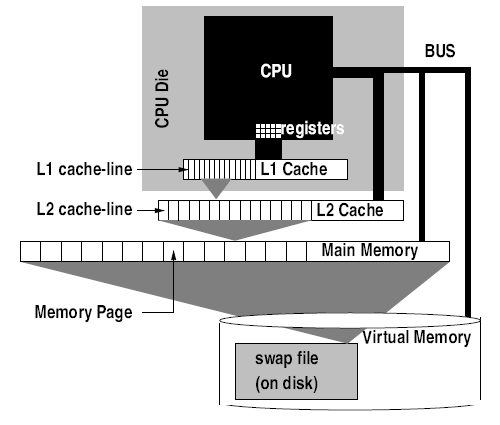
\includegraphics[width=0.4\textwidth]{./pictures/Fig1}
  \end{center}
  \caption{Hierarchical Memory System}
\end{wrapfigure}

Hard Disk drives are the cheaper, scalable and reliable solution for data storage but due to mechanical parts involved in the data access it has considerable latency issues as compared to other storage media and thus lies at the bottom of the storage hierarchy in terms of performance (Figure 1).

RAM or DRAM lies below high speed L1/L2 cache or SRAM but above any other storage medium in memory hierarchy system categorized as increase in performance from bottom to top as shown in figure 1. Since the SRAM cannot be extended in size due to hardware limitations therefore DRAM or RAM is the ideal candidate for data storage.

Solid State Drives (SSDs) are nowadays another popular and widely used data storage devices in systems all over the world. Embedded and real time systems and even personal computers and laptops utilize their low latency data access features for specific applications. Since no moving part is included in SSDs, they outperform the hard disks in terms of disk I/O operations resulting in better responsiveness \cite{Mcobject-Myths}. Even though these NAND based devices are faster and better in performance than hard disks but they are nowhere near to DRAMs amazing speeds \cite{ssds}. 

\begin{description}
  \item[Definition] As the name implies Main Memory Databases MMDB or In Memory Databases (IMDB) is a database management system which stores the complete database on physical memory or RAM. 
\end{description}

\subsection{History}
Most people argue in memory computing to be a relatively new and unproven technology. This is a myth rather than fact. For ages caching mechanisms is being used in traditional DRDBs which involves the most frequent use data inside RAM for fast access \cite{Mcobject-Myths} . In addition in-memory tables feature have also been part of some DBMS to hold data inside Main Memory. Also the use of DRDBs in main memory was a practice carried out to get better response times. 

This entails that MMDB are not new and considerable work has been done in this regard in 1980s. However they were not popular as the cost of memory and other limitations related to persistence of data were considered a problem. Many experimental MMDBs were developed then like MARS, HALO and MM-DBMS as part of research along with commercial systems like IBM Fastpath \cite{garcia1992main}. 

As of today IBM, Oracle and SAP being the top database vendors in the market have acquired the companies which were developing and marketing in memory database solutions \cite{pressRgiants}. Gartner\footnote{Gartner, Inc. is an American information technology research and advisory firm head-quartered in Stamford, Connecticut, United States} has placed In Memory computing as part of \emph{Top ten technology trends for 2013} \cite{gartner}. This clearly indicates the increase in the demand of MMDBs in market and their adaptation to the solutions in coming years.  

\subsection{Bounds of MMDBs}
MMDBs with their high performance mechanisms are the perfect contenders for embedded systems \cite{graves2002memory}. These systems with the evolution of smarter devices and expanding feature set needs to manage complex data structures which while written from ground up will require extra effort. With MMDBs pointer style low latency data access and simpler optimization techniques the embedded system developers have less things to worry about, stepping MMDBs adaptation to these types of systems. These systems include set-top boxes, network switches and consumer electronics. 

The real-time systems require time-critical access to and processing of massive amounts data. Example applications that handle large amounts of data and have stringent timing requirements include telephone switching, radar tracking and others. Furthermore as stated by \cite{ilprints39}, the real time database system design must not contain latency components like disk I/O operations, massage passing or garbage collection. Thus MMDBs architecture fits perfectly into the real-time application scenario. 

The role of the MMDBs has greatly expanded over the last couple of years as high-end 64-bit servers can now accommodate databases that are quite large – even terabytes in size. Therefore the applications for large IMDBs further include many popular large-scale Web applications and social networking sites. 

Nowadays, the data within an enterprise is distributed throughout a wide range of applications and stored in disjoint locations. Analytical reporting with amalgamated view on the data as a whole is a cumbersome and time-consuming process. Besides these reports are not entirely based on the operational data, but on combined data from a data warehouse by transforming it through ETL\footnote{ETL (Extract, Transform and Load) is a process in data warehousing responsible for pulling data out of the source systems and placing it into a data warehouse}process. Hasso has pointed out in \cite{plattner2011memory} that In-Memory data management assists the analytical operations resulting in planning, forecasting and faster decision making by separating it from operational data processing. Thus resulting in innovative and hybrid style of enterprise applications residing partially or fully in memory. 

%------------------------------------------------------------------------------------
%	Background and Analysis <-- TODO: is the name for this section accurate? 
%------------------------------------------------------------------------------------
% Let's talk about the main topic in terms of three major parts:
% - Data Organization
% - Query Processing
% - Data Recovery

\section{MMDB vs. DRDB : A Comparison}
A Main Memory Database Management System eliminates the most expensive Disk I/O operations which are the bottle neck in traditional DRDBs. The complete database resides inside RAM. However the question here arises \emph{Putting a DRDB in main memory will deliver us the same performance results as a MMDB} or \emph{MMDBs are the same traditional databases inside RAM}. This notion is not true at all. Although the traditional DRDB inside main memory out performs its instance on disk but while its comparison with pure MMDB the performance gap is far too much \cite{Mcobject-ramdisk}. Linux systems and now windows as well have the capability to create a RAM disk (File system inside the main memory). But a traditional DRDB deployed on such a virtually fast hard drive doesn't provide the same benefits of a pure MMDB. In-memory databases are less complex than their on disk counterparts fully deployed in physical memory and thus require minor usage of processing cycles and RAM.

Another popular feature which most database providers provide in their DBMSs are the creation of memory tables, through which certain tables can be designated for all-in-memory handling \cite{Mcobject-Myths}. So does this mean that \emph{with these memory features, DRDBs can compete with MMDBs performance?}. Not really as the problem remains the same as memory tables not only don't change the database design assumptions but also have certain additional restrictions. For example, in MySQL, memory tables cannot contain BLOB or TEXT columns and the maximum table size is fixed. Furthermore in contrast to MMDBs, the space that is freed up by deletion of tuples in an in-memory relation can only be used by the same relation, which is wastage of precious space inside RAM.

Comparing MMDBs with DRDBs we can find at least 4 key differences:

\begin{itemize}
\item Cache Maintenance
\item Data Transfer
\item Transaction Logging
\item Concurrency Control 
\end{itemize}

\subsection{Cache Maintenance}
\subsection{Data Transfer}
\subsection{Transaction Logging}
\subsection{Concurrency Control}
\section{Characteristics/Strong points of MMDB}
\section{Issues in MMDBs}



\section{Background and Analysis} 
\subsection{Concepts}
We need to put concepts, I've found a good source from (\citeA{Kemper})

\subsection{Technology awareness}
Let's put here something related with the main concerns that leads to this emerging technology. Also, its important to be aware that the ACID properties of DB Systems should be contrasted. In terms of each one of its meanings.

\begin{description}
    % this ideas are collected from Kemper
  \item[Atomicity] In order to achieve atomicity, the IMDB should be able to handle the effects of unsuccessful transactions. In general terms, the problem has to explicitly with the data existent in the volatile memory, since all successful transaction are in a successful state only after been committed to the logging infrastructure. % <-- PV remember, atomicity is all or nothing.
  \item[Durability] It is clear that during a failure, the IMDB Systems has the most obvious disadvantage, (without mention the hardware based solutions like batteries and so on), so the effects of a commit must be restored on a failure, this is the principle of Durability of course. One of the ideas to accomplish this is use \emph{ redo Logging }. %<-- PV important, should be more, worth to investigate 
\end{description}


% IVAN: New content added from the new task split between our team mates:
% - My part begins with Indexing, this is not part of the data organization??, yes so I shall start with data organization.
% - Actually it is, because we have organized the structure as this document know explains, follow this document structure please.


\section{Data Organization}

Relational Databases have been the backbone of business applications for more  than 20 years, trying to provide companies with a management information system for a set of applications. During all this time, we have dreamed with the possibility of having all the information at our fingertip, we even have sold this idea\cite{Plattner}.

    But due to many reasons, we have not been able to offer this. And our systems have been separated in two main different groups: The online transaction processing (OLTP) and on line analytical processing (OLAP).

\subsection{OLTP and OLAP}
    % from \cite{Kemper}
    Under the OLTP classification, could be grouped systems with a high rate of day to day transactions, most of the database systems (as we know them) are mainly used for transaction processing. Some examples of OLTP systems are financial, sales, Manufacturing, order entry, banking transaction processing, human resources. All this systems performs relatively well mainly because they work on a small portion of the data. The TCP-C benchmark publish an average processing of 100.000 such sales transactions per second on a powerful system \cite{Kemper}.
    
    On the other hand, analytical, business intelligence and financial planning application were moved out to separated systems (for more flexibility and better performance). The OLAP Systems could be aimed toward specific task related to the company data warehousing. 
    
    Even though, this solutions are different in context, both are still based on \emph{ Relational theory } but with different technical approaches. The main purposes of this separation could be generalized into \emph{ performance } and maybe \emph{technical} issues. Even though both systems keep the essence in terms of relational theory, there are some important differences between them \cite{Plattner}.

    Moreover, recent development in the field of OLAP and the increased availability of main memory (sufficient enough to hold a completed compressed database) have enabled the processing of complex analytical requests in a fraction of a second and thus ease the development of new business processes and applications. The next step seems obviously to undo the separation between OLTP and OLAP and all requests be handled on a combined data set.

    %TODO: should I keep adding more info here? we can still talk about OLAP cubes, etc

    Now that the main memory is abundant, we have gone back to see the possibility of having a all-in-one MMDB. SAP\footnote{SAP AG: A German multinational software corporation that makes enterprise software to manage business operations and customer relations.} is one of the most enthusiastic companies pushing the use of Main Memory Databases for a mixed OLTP \& OLAP environment \cite{Plattner}, the company advertises SAP HANA as a generic MMDB solutions. 
    
    In this direction, it is suitable to estimate the challenges toward this join in technical perspectives, specifically, we have defined two main critical points related to data organization: The improved MMDB indexing system and the data Storage.

    
\subsection{MMDB Indexing}
It is mandatory to talk first about the differences between MMDB and on-disk DB, at first instance: In a MMDB Index, the main goal is to redesign the data structure and algorithm to make efficient use of \emph{ CPU } and \emph{ memory space } rather than minimize disk access, since we don't have disk of course. On the other hand, disk-oriented index structure are designed to minimize disk access and minimize disk space, this mainly because traditional database systems are CPU bounded because they spend considerable effort to avoid disk accesses.

A Main Memory oriented index structure is designed to reduce overall computation while using as little memory as possible \cite{lehman1986study}, since everything is in memory, MMDB Index could store only pointers to tuples or structures in the main memory (the actual data) instead of storing attribute values as on-disk DB usually does, decreasing efficiently the index footprint.

 Although a MMDB system could be arranged in different ways, two main types of \emph{ Main Memory Index Structure } could be specified: Order Preserving index structures and randomized \cite{lehman1986study}. Under the order preserving group could be summarized: arrays, AVL Trees, B Trees and T-Trees. T-Tree is one of the most important and well know structure, named T-Tree after its 'T' shape. On the other randomized group falls: Chained Bucket Hashing, Linear Hashing and Extendible Hashing.

Although, the performance observed in a MMDB could be outstanding compared to a on disk DB, the index structure is a critical bottleneck \cite{leisadaptive}. The T-Tree (and one of the most developed) index technology involved in MMDB was proposed 25 years ago, and was designed based on the AVL and B Trees. Acording to \citeA{leisadaptive}, ``the dramatic processor architecture changes have rendered T-trees, like all traditional binary search trees, inefficient on modern hardware''.

TODO: maybe talk about details of t-trees\ldots 
% PV TODO: in lehman1986study there is more info about indexing and a detailed explanation of t-tree and its derived


\subsubsection{Column-Store Database System}

Column-oriented databases are based on vertical partitioning by columns, this is not a new idea, Column-oriented store where considered around 70s. The core of the functioning is based in the fact that each column is stored separately, having the logical scheme built around unique positioning keys \cite{krueger2011main}. This vertical data organization offers particular advantages to reading fewer attributes. According to \cite{Plattner}, in real world applications, ``only 10\% of the attributes of a single table are typically used in one SQL statement'', this could imply that: if during requests no unnecessary columns must be read, we could just use the columns independently of the related column attributes. Row oriented structures on hard drives normally can't perform this independence.

As a first premise, recent improvements in parallel processing of modern CPUs, could lead to think that a column oriented approach today seems to be ideal. The Column oriented storage has the following advantages: 

\begin{itemize}
  \item Column Store performs outstanding on modern CPUS.

  \item The Storage model is based on vertical fragmentation.

  \item Column Store Allow data compression

  \item Better memory consumption performance

  \item Data arranged in columns are better suited for parallel processing because of its independence.

\end{itemize}
   
Although, column oriented storage presents a lot of interesting features, it's worth to mention that there are also some drawbacks that kept this technology behind row oriented storage: for example: Column stores are expensive to update, but also having all data in main memory overcomes this limitation. Also column store increases seek time, but this is a concern only for on-disk DB systems.

From \cite{Plattner}, it seems that although more memory has been always useful, the database systems for OLTP where not well adopted in parallel environments, one of the reasons of this were problems like deadlocks and temporary locking in parallel transactions. So in general terms has not been a good idea. Really? review this since Plattner is one of the pro Column Oriented store.

Also from \cite{Plattner}, initial tests regarding in-memory databases using relational type based on \emph{ row storage } has not shown notable performance over RDBMSs. The opportunity for \emph{column based storage} now raises due the abundant availability of main memory. 

Compression is another characteristic that Column-oriented ease. The redundancy of column store and the homogeneous domain is an advantage and a convenience for compression techniques. All the data within a column belongs to the same type, and the entropy\footnote{The entropy could be defined as the similarities of data} is relatively low. 

TODO: talk more about column oriented, put some graphics

\subsection{IMDB Data Recovery}

% PV: stupid idea: the memory comsumption is high since IDBM is memory based, but, OS Systems like Unix uses as much memory as they can in order to be more efficient, after coping all the memory, they start to swap and problems like trashing could happen.
% PV: stupid idea2: In a computer, all the memory has to be used because is already payed, the resource is there so take as much memory as you can.

\section{Conclusions} 

% This is the point about conclusions and future directions
\subsection{Conclusion regarding OLTP and OLAP merging}




We could talk about: \emph{ MonetDB }, \emph{ VoltDB }


%------------------------------------------------------------------------------------
%	BIBLIOGRAPHY
%------------------------------------------------------------------------------------
% This is the part about references

\bibliographystyle{apacite}
\bibliography{bibfile}
%------------------------------------------------------------------------------------
\end{document}
